\documentclass[12pt, letterpaper]{article}
\usepackage{graphicx}
\usepackage{float}
\usepackage{cclicenses}
\usepackage{hyperref}
\usepackage{textcomp}

\setlength\parindent{0pt}

\begin{document}

\begin{titlepage}
\title{LaptopAlarm Help}
\author{Ethan Nguyen}
\date{Updated April 22, 2018}
\maketitle
\thispagestyle{empty}

\vfill

\url{https://www.github.com/etnguyen03/LaptopAlarm} \\
\url{http://www.ethannguyen.tk}
\\
\\
\textcopyright{} 2018 Ethan Nguyen; some rights reserved. \\
This document is licensed under the Creative Commons Attribution-ShareAlike 4.0 International license. \\

\url{https://creativecommons.org/licenses/by-sa/4.0/}

\end{titlepage}

\tableofcontents
\pagebreak

\part{Basic Usage}
\section{Arming and Disarming}
Arming is performed by pressing CTRL + ALT + A. A tray message will confirm arming. You can only arm LaptopAlarm while you are logged in to Windows.

Be aware that arming the alarm while the power cord is removed or the battery is disconnected (if enabled in settings) will immediately trigger the alarm.

By default, the alarm is triggered when the laptop's power cord is disconnected.

\begin{figure}[H]
  \caption{Arming tray message}
  \centering
    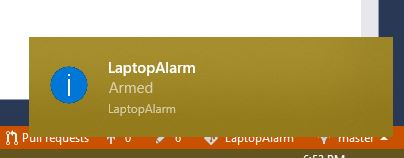
\includegraphics{figures/figure01.JPG}
\end{figure}

Disarming is performed by pressing CTRL + ALT + D. A tray message will confirm disarming. You can only arm LaptopAlarm while you are logged in to Windows. To prevent others from disarming LaptopAlarm, it is recommended that you have a password lock on your user account and lock (WINDOWS + L) to lock your account.

\begin{figure}[H]
  \caption{Disarming tray message}
  \centering
    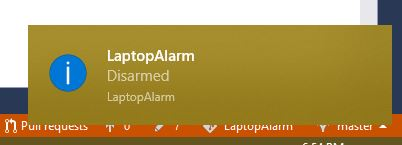
\includegraphics{figures/figure02.JPG}
\end{figure}

\section{Cancelling an alarm}

Should an alarm be triggered, an ``ALARM'' dialog box will show and a tray notification will be displayed. To cancel the alarm, you must be signed into your account (you cannot be on the Windows lock screen). Then, press CTRL + ALT + D or disarm the alarm from the context menu.

\begin{figure}[H]
  \caption{Alarm tray notification}
  \centering
    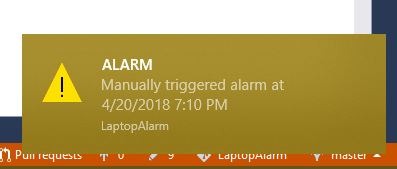
\includegraphics{figures/figure04.JPG}
\end{figure}

\begin{figure}[H]
  \caption{Alarm dialog box}
  \centering
    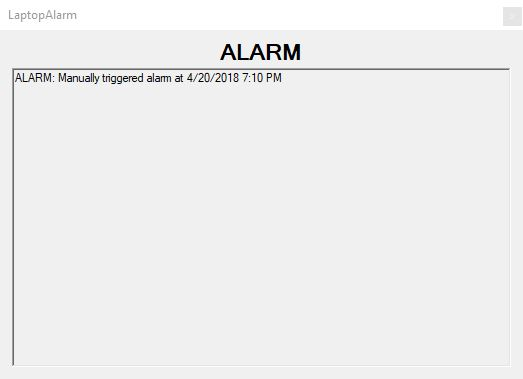
\includegraphics{figures/figure05.JPG}
\end{figure}

\section{Tray Icon Context Menu}
Right clicking LaptopAlarm's tray icon will show a context menu. From this menu, you can arm or disarm the alarm, trigger the alarm in panic situations, show LaptopAlarm's configuration options, or exit LaptopAlarm.

\begin{figure}[H]
  \caption{Tray Icon Context Menu}
  \centering
    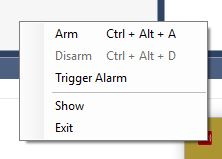
\includegraphics{figures/figure03.JPG}
\end{figure}

\subsection{Triggering Alarm}
You can immediately trigger the alarm from the right-click context menu. You can use this feature in case of panic. You can remove this option from the context menu from the ``Program Settings'' tab in the settings window.

\part{Customizing Settings}
\section{Accessing the Settings Window}
To access the LaptopAlarm settings window, right-click the LaptopAlarm tray icon and select ``Show''. LaptopAlarm's settings page will show.

\begin{figure}[H]
  \caption{Settings window}
  \centering
    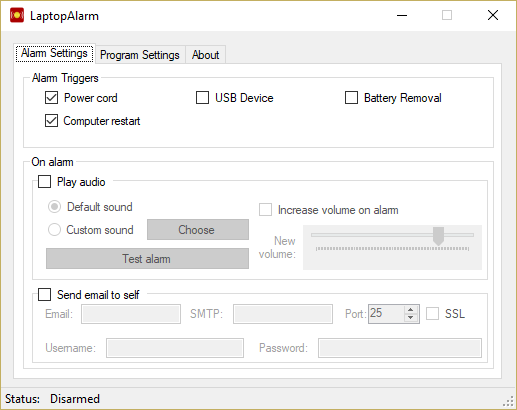
\includegraphics{figures/figure06.png}
\end{figure}

\section{Alarm Settings}
\subsection{Alarm Triggers}
This section alters when LaptopAlarm will trigger the alarm.
\paragraph{Power cord}
If this option is selected, LaptopAlarm will trigger the alarm when the power cord is disconnected. Be aware that arming the alarm when the power cord is disconnected will cause an alarm.
\paragraph{USB Device}
If this option is selected, LaptopAlarm will trigger the alarm whenever any USB device is disconnected.
\paragraph{Battery removal}
If this option is selected, LaptopAlarm will trigger the alarm whenever the laptop's battery is removed. Be aware that arming the alarm when the battery is removed will cause an alarm.
\paragraph{Computer restart}
If this option is selected, LaptopAlarm will trigger the alarm whenever the computer is restarted. LaptopAlarm must be configured to startup on computer startup for this to happen (see ``Program Settings'' tab).

\section{On Alarm}
\subsection{Play Audio}
\paragraph{Sounds}
You can select the sound that LaptopAlarm will play when the alarm is triggered. The default sound is a burglar alarm sound. You may specify a custom sound by selecting ``Custom Sound'' and choosing a .wav file.
\paragraph{Increase Volume on Alarm} LaptopAlarm, by default, will increase and lock the computer volume at 80\%. You may specify a different audio volume, or turn off the feature entirely.
\paragraph{Test alarm} Clicking this button will sound the alarm. This button will not increase the volume.

\subsection{Send email to self}
This feature has not been tested. If this option is enabled, LaptopAlarm will send an email to the email address you specify.
\paragraph{SMTP Settings} These are settings provided by your email provider. Check with them for more details.

\section{Program Settings}

\begin{figure}[H]
  \caption{Program Settings tab}
  \centering
    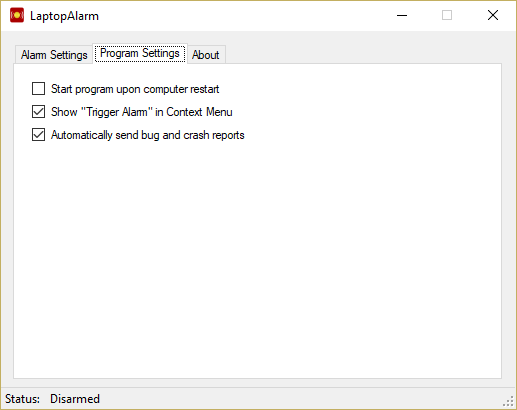
\includegraphics{figures/figure07.png}
\end{figure}

\subsection{Start program on computer restart}
This option does not work. It is currently being worked on.

\subsection{Show ``Trigger Alarm'' in Context Menu}
If this option is selected, the option ``Trigger Alarm'' is shown in the right-click context menu.
By default, this option is selected.

\subsection{Automatically send bug and crash reports}
If this option is selected, LaptopAlarm will automatically send bug and crash reports to the developer when one is encountered.

\end{document}
